\documentclass[]{elsarticle} %review=doublespace preprint=single 5p=2 column
%%% Begin My package additions %%%%%%%%%%%%%%%%%%%
\usepackage[hyphens]{url}
\usepackage{lineno} % add
\providecommand{\tightlist}{%
  \setlength{\itemsep}{0pt}\setlength{\parskip}{0pt}}

\bibliographystyle{elsarticle-harv}
\biboptions{sort&compress} % For natbib
\usepackage{graphicx}
\usepackage{booktabs} % book-quality tables
%% Redefines the elsarticle footer
%\makeatletter
%\def\ps@pprintTitle{%
% \let\@oddhead\@empty
% \let\@evenhead\@empty
% \def\@oddfoot{\it \hfill\today}%
% \let\@evenfoot\@oddfoot}
%\makeatother

% A modified page layout
\textwidth 6.75in
\oddsidemargin -0.15in
\evensidemargin -0.15in
\textheight 9in
\topmargin -0.5in
%%%%%%%%%%%%%%%% end my additions to header

\usepackage[T1]{fontenc}
\usepackage{lmodern}
\usepackage{amssymb,amsmath}
\usepackage{ifxetex,ifluatex}
\usepackage{fixltx2e} % provides \textsubscript
% use upquote if available, for straight quotes in verbatim environments
\IfFileExists{upquote.sty}{\usepackage{upquote}}{}
\ifnum 0\ifxetex 1\fi\ifluatex 1\fi=0 % if pdftex
  \usepackage[utf8]{inputenc}
\else % if luatex or xelatex
  \usepackage{fontspec}
  \ifxetex
    \usepackage{xltxtra,xunicode}
  \fi
  \defaultfontfeatures{Mapping=tex-text,Scale=MatchLowercase}
  \newcommand{\euro}{€}
\fi
% use microtype if available
\IfFileExists{microtype.sty}{\usepackage{microtype}}{}
\usepackage{graphicx}
% We will generate all images so they have a width \maxwidth. This means
% that they will get their normal width if they fit onto the page, but
% are scaled down if they would overflow the margins.
\makeatletter
\def\maxwidth{\ifdim\Gin@nat@width>\linewidth\linewidth
\else\Gin@nat@width\fi}
\makeatother
\let\Oldincludegraphics\includegraphics
\renewcommand{\includegraphics}[1]{\Oldincludegraphics[width=\maxwidth]{#1}}
\ifxetex
  \usepackage[setpagesize=false, % page size defined by xetex
              unicode=false, % unicode breaks when used with xetex
              xetex]{hyperref}
\else
  \usepackage[unicode=true]{hyperref}
\fi
\hypersetup{breaklinks=true,
            bookmarks=true,
            pdfauthor={},
            pdftitle={Fitting a Random Linear Preferential Attachment Model for Directed Graphs},
            colorlinks=true,
            urlcolor=blue,
            linkcolor=magenta,
            pdfborder={0 0 0}}
\urlstyle{same}  % don't use monospace font for urls
\setlength{\parindent}{0pt}
\setlength{\parskip}{6pt plus 2pt minus 1pt}
\setlength{\emergencystretch}{3em}  % prevent overfull lines
\setcounter{secnumdepth}{0}
\setlength\parindent{24pt}
\usepackage{graphicx}
% Pandoc toggle for numbering sections (defaults to be off)
\setcounter{secnumdepth}{0}
% Pandoc header
\setlength\parindent{24pt}
\usepackage{graphicx}


\usepackage[nomarkers]{endfloat}

\begin{document}
\begin{frontmatter}

  \title{Fitting a Random Linear Preferential Attachment Model for Directed
Graphs}
    
  \begin{abstract}
  The text of your abstract. 200 or fewer words.
  \end{abstract}
  
 \end{frontmatter}

\subsection{Introduction}\label{introduction}

A well-discussed property thought to be common among the degree
distribution of networks is that it obeys a power law distribution.
Namely, let \(f(d)\) be the fraction of nodes with degree \(d\), then
\[f(d) \propto d^{-\alpha}, \ \  \text{ for } d \geq d_{\min}\]
\(\alpha > 1\) is said to be the power law exponent. The distribution
has infinite first moment when \(1 < \alpha < 2\), infinite
second-moment when \(2 < \alpha < 3\). It is dubbed interchangeably
between networks which have a power law degree distribution and networks
which are ``scale-free'' since power law is the only functional form
which satifies scale-invariance,
\[f(cd) \propto (cd)^{-\alpha} = c^{-\alpha}d^{-\alpha} \propto f(d)\]
for some constant \(c\). In order to give some theoretical underpinning
to the seemingly wide-spread phenomena of scale-free networks, Barabási
and Albert (1999) proposed the following simple canonical linear
preferential attachment (PA) model for undirected, unweighted networks.
Let \(\{G(t) \}_{t = t_0}^{T}\) be a sequence of graphs indexed by time
\(t\). Let \(G(t_0)\) be the initial given graph with \(m_0\) nodes.
Then at each \(t > t_0\), generate \(G(t)\) from \(G(t-1)\) by adding a
new node, \(v\), and form an edge between \(v\) and each of the
\(m (\leq m_0)\) existing nodes, with the probability proportional to
the node degree,
\[\mathbb{P}[\text{ choose }w \in G(t-1)] = \frac{{k_w}^{\alpha}}{\sum_j{ k_j}^\alpha}, \ \ \alpha = 1\]
where \(k_w\) is the degree of node \(w\). It is linear because
\(\alpha =1\). Such linear PA mechanism would generate the
``rich-get-richer'' effect, and as rigorously proved in Bollobás et al.
(2001), in the limit, \(f(d) \sim Cd^{-\alpha}\) with \(\alpha = 3\).
However, Krapivsky, Redner, and Leyvraz (2000) has shown that under this
model, the network is only scale-free if \(\alpha = 1\): if
\(\alpha < 1\) then the limiting degree distribution is streched
exponential; if \(\alpha > 1\) we would get winner take all - one node
that connects to nearly all other nodes. Many growth models have been
subsequently proposed which generate scale-freeness in the limit, some
use a preferential attachment mechanism and some not, and often require
model parameters to fall on some range or exact point, see Table 3 of R.
Albert and Barabasi (2001) for a summary of analytical results.

Most work on testing for the scale-freeness of networks have been
exclusively on determining whether the resulting degree distribution
obeys power law, not fitting the hypothesized growth model. However, as
Broido and Clauset (2018) have pointed out, many such works rely on less
rigorous statistical methods as fitting fat-tailed distributions is
difficult, and often used small sample datasets. Moreover, likelihood
ratio tests are seldem done to compare power law to other fat-tailed
distributions. This is crucial as illustrated by the
Barabasi-Albert-type model, streched exponential and power law are all
possible limiting distributions and the parameter requirement for
scale-freeness is exact.

Besides the statistical concerns, stricly analyzing the resulting degree
distribution is fundementally not a network problem. In order to
understand the network processes which could generate scale-freeness, it
would be of great benefit to directly fit the underlying process to
provide another tool-kit to analyze the formation of degree
distribution. However, most work on fitting growth models rely on having
the entire history of the graph process, relatively few (Wiuf et al.
2006, Bezáková, Kalai, and Santhanam (2006), Bloem-Reddy and Orbanz
(2016), Guetz and Holmes (2011), Leskovec et al. (2010), Wan et al.
(2017)) developed methods to fit growth models based on a single
snapshot, which significatly limited the number of datasets that
researchers can analyze. Therefore, the goal of this paper is to fit a
network growth model based on a single snapshot of the graph and conduct
simulation and predictive checking studies to see how well the model
explains the empirical degree distribution of the network.

The model I will be fitting is a 5-parameter linear preferential
attachment model for directed, unweighted network, described below.

\subsection{The Model}\label{the-model}

\begin{figure}[htbp]
\centering
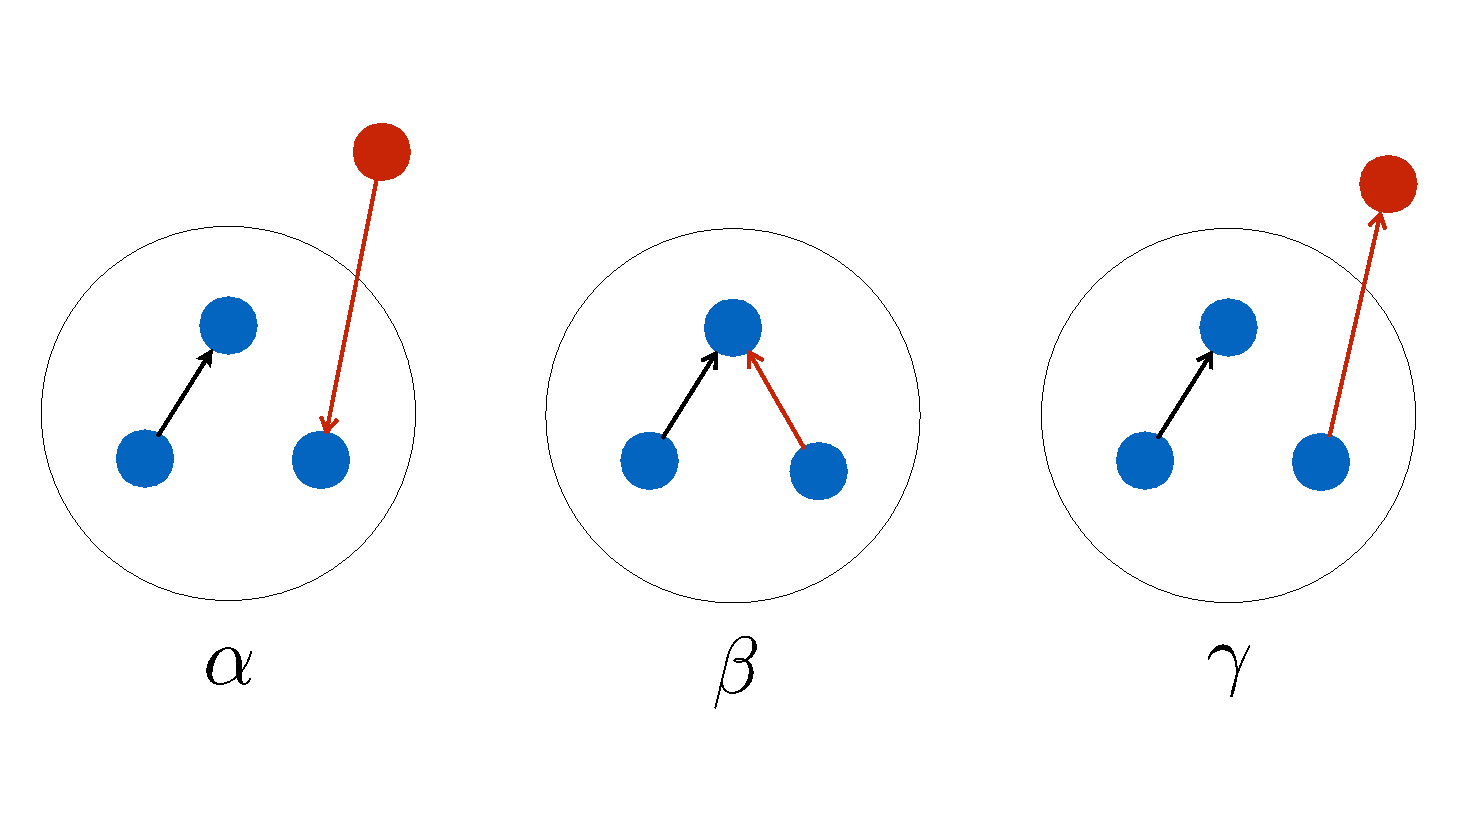
\includegraphics[width=4.47917in]{/Users/MacUser/Desktop/Network/Final Project/scheme.pdf}
\caption{Edge/Node-Addition Schemes}
\end{figure}

The model is a random linear PA model for directed graphs as described
in Bollobás et al. (2003), with the parameter vector with all positive
elements
\(\boldsymbol{\theta} = (\alpha, \beta, \gamma, \delta_{in}, \delta_{out})\).
As usual, \(G(n) = (V(n), E(n))\), where \(V(n)\) denotes the set of
nodes at time \(n\) and \(E(n)\) denotes the set of edges at time \(n\).

For this linear PA model, at \(n+1\) an \emph{edge} is added to \(G(n)\)
to form \(G(n+1)\). Following the notation in Wan et al. (2017), let
\(n \equiv | E(n)|\), where \(| \cdot |\) denotes the cardinality, and
let \(N(n) \equiv |V(n)|\). For every
\(u \in V(n), \ D_{in}^{(n)}(u) \text{ and } D_{out}^{(n)}(u)\) denotes
the in- and out-degree of \(u\) in \(G(n)\), respectively. Let
\((v, w)\) denote a directed edge from \(v\) to \(w\). We assume that
there is a given initial finite directed graph \(G(n_0)\) with at least
one node and \(n_0\) edges. For all \(n > n_0\) and given \(G(n-1)\),
generate \(G(n)\) as follows,

\begin{enumerate}
\def\labelenumi{\arabic{enumi}.}
\tightlist
\item
  Toss a three-sided coin \(J_n\) with \(\Omega = \{1, 2, 3\}\) and the
  following mass function,
  \(\mathbb{P}(J_n = 1) = \alpha, \ \mathbb{P}(J_n = 2) = \beta, \ \mathbb{P}(J_n = 3) = \gamma\).
  Assume \(0 < \alpha, \ \beta,\ \gamma < 1\) to avoid degeneracy.
  \(\{ J_n \}\) then forms a multinomial process.
\end{enumerate}

\begin{itemize}
\item
  If \(J_n = 1\) (\(\alpha\)-scheme): Add a new node, \(v\), to
  \(G(n-1)\) and an edge \((v, w)\) leading from \(v\) to a previously
  existing \(w \in V(n-1)\). The choice of \(w\) is based on the
  following probability,

  \begin{align}
  \mathbb{P}[\text{ choose } w \in V(n-1)] = \frac{ D_{in}^{(n-1)}(w) + \delta_{in} }{n - 1 + \delta_{in}N(n-1)}
  \end{align}

  That is choose \(w\) with the probability proportional to its
  in-degree and corrected by a bias parameter \(\delta_{in}\)
\item
  If \(J_n = 2\) (\(\beta\)-scheme): Add a directed edge \((v, w)\) to
  \(E(n-1)\) where \(v, w \in V(n-1)\) (no new node is added). Choose
  \((v, w)\) as such,

  \begin{align}
  \mathbb{P}[\text{choose } (v, w)] = \Big(\frac{ D_{in}^{(n-1)}(v) + \delta_{in} }{n - 1 + \delta_{in}N(n-1)} \Big) \Big( \frac{ D_{out}^{(n-1)}(w) + \delta_{out} }{n - 1 + \delta_{out}N(n-1)}\Big)
  \end{align}

  In other words, \(v\) and \(w\) are being chosen independently and the
  probability of \(w\) being chosen is proportional to its in-degree and
  the probability of \(v\) being chosen is proportional to its
  out-degree.
\item
  If \(J_n = 3\) (\(\gamma\)-scheme): Add a new node \(w\) to \(G(n-1)\)
  and an edge (v, w) leading from an existing node \(v\) to \(w\) with
  the probability,
\end{itemize}

\begin{align}
\mathbb{P}[\text{ choose } v \in V(n-1)] = \frac{ D_{out}^{(n-1)}(v) + \delta_{out} }{n - 1 + \delta_{out}N(n-1)}
\end{align}

Figure 1 shows the edge-addition schemes based on the coin toss. In
summary: in the \(\alpha\)-scheme, add a new node and directs it to an
existing node where the existing node is being chosen proportional to
its in-degree; in the \(\beta\)-scheme, no new node is added, but add a
new edge between two existing node with the probability as being
proportional to the product of their in and out-degrees; in the
\(\gamma\)-scheme, add a new node, and direct an existing node to the
new node added, where the existing node is being chosen proportional to
its out-degree.

\subsubsection{Power law as the limiting degree
distribution}\label{power-law-as-the-limiting-degree-distribution}

Bollobás et al. (2003) studied the limiting in- and out-degree
distribution of this model and showed that the marginal in and
out-degree distribution of the graph has the power law property in the
following way. Let \(x_i(n)\) denote the number of nodes in \(G(n)\)
with in-degree \(i\), so \(x_i(n)/{N(n)}\) is the fraction of nodes with
in-degree \(i\) at time step \(n\). Similarly, let \(y_i(n)\) denote the
number of nodes in \(G(n)\) with out-degree \(i\), and write
\(y_i(n)/N(n)\). Then by Theorem 3.1 of Bollobás et al. (2003), there
exists constants \(p_i, q_i\) for fixed \(i \geq 1\) such that as
\(n \to \infty\), almost surely

\begin{align}
\frac{x_i(n)}{N(n)} \rightarrow p_i, \ \ \frac{y_j(n)}{N(n)} \rightarrow q_i
\end{align}

\noindent See equation 3.10 of Bollobás et al. (2003) for the closed
form solution of \(p_i\) and \(q_i\). Then taking the limit as
\(i \to \infty\),

\begin{align}
p_i \sim C_{1} i^{\kappa_{in}}  \ \ \text{    if } \alpha \delta_{in} + \gamma > 0, \ \ \ \kappa_{in} = 1 + \frac{1+ \delta_{in}(\alpha + \gamma)}{\alpha + \beta} \\
q_i \sim C_{2} i^{\kappa_{out}}  \ \ \text{    if } \gamma \delta_{out} + \alpha > 0, \ \ \ \kappa_{out} = 1 + \frac{1+ \delta_{out}(\alpha + \gamma)}{\beta + \gamma}
\end{align}

\noindent where \(C_{1}, C_{2}\) are positive constants and
\(f_i \sim g_i\) denotes \(f_i/g_i \to 1\) as \(i \to \infty\).

\subsubsection{Parameter Estimation, Inference, and
Simulation}\label{parameter-estimation-inference-and-simulation}

Wan et al. (2017) has proposed a MLE approximation procedure to estimate
\(\boldsymbol{\theta}\) just based on a single snapshot of the graph.
Let \(X_{> i}(n) = \sum_{j > i}x_{j}(n)\) and
\(Y_{>i}(n) = \sum_{j > i} y_j(n)\) denote the number of nodes with
in-degree greater than \(i\) in \(G(n)\) and the number of nodes with
out-degree greater than \(j\) in \(G(n)\), respectively. Let
\(\boldsymbol{\tilde{\theta}}\) be the estimator for
\(\boldsymbol{\theta}\). Then Wan et al. (2017) p.13-14 proposed a
simple algorithm to compute \(\boldsymbol{\tilde{\theta}}\) where
\(\boldsymbol{\tilde{\theta}}\) is strongly consistent, i.e.
\(\boldsymbol{\tilde{\theta}} \overset{a.s.}{\to} \boldsymbol{\theta}\)
element-wise. I won't outline the complete derivation here, but the
basic idea is that, as they have shown, \(\{ X_{> i}(n) \}_{i}\),
\(\{ Y_{>i}(n) \}_{i}\), and \(\{ J_n \}_{n}\) (the multinomial coin
process) are sufficient statistics for \(\boldsymbol{\theta}\), but
\(\{ J_n \}_n\) is unknown from a single snapshot. However,
\(\boldsymbol{\theta}\) can in fact be well-approximated by functions of
\(\{ X_{> i}(n) \}_{i}\) and \(\{ Y_{>i}(n) \}_{i}\) only, if \(n\) is
large. The result is that
\(\tilde{\alpha}, \tilde{\beta}, \tilde{\gamma}\) can be computed in
closed-form, with \(\tilde{\beta} = 1 - N(n)/n\) which intuitively makes
sense, and obtaining \(\tilde{\delta}_{in},\ \tilde{\delta}_{out}\) each
requires numerically solving an implicit function. The authors suggested
a procedure to re-normalize \(\tilde{\boldsymbol{\theta}}\) so that
\(\tilde{\alpha} + \tilde{\beta} + \tilde{\gamma} = 1\). It should be
noted that from my experience, without the re-normalization procedure
\(\tilde{\delta}_{in}\) and \(\tilde{\delta}_{out}\) are not guaranteed
to be strictly positive, as assumed by the model.

As for inference, there are no formal inference procedure propsed,
instead the authors suggested the following bootstrapping procedure to
estimate the variance of \(\boldsymbol{\tilde{\theta}}\). Use
\(\boldsymbol{\tilde{\theta}}\) to simulate \(10^4\) independent
bootstrap replicates of network with \(n = 10^5\) edges. For each
simulated network, compute the snap-shot esimate
\(\boldsymbol{\tilde{\theta}_n^*} \equiv (\tilde{\alpha}^*, \tilde{\beta}^*, \tilde{\delta}_{in}^*, \tilde{\delta}_{out}^*)\)
and take the sample variance,
\(\hat{\text{Var}}(\boldsymbol{\tilde{\theta}_n^*})\), of
\(\boldsymbol{\tilde{\theta}_n^*}\) over the \(10^4\) snap-shot
estimates to approximate \(\text{Var}(\boldsymbol{\tilde{\theta}})\).
Then by assuming asymtotic normality, construct the two-sided confidence
interval of \(( 1 - \epsilon)\) as usual,
\[\{ \boldsymbol{\tilde{\theta}_n}\}_{i} \pm z_{\epsilon/2}\sqrt{\hat{\text{Var}}(\{ \boldsymbol{\tilde{\theta}_n^*}\}_{i})}, \ \ \ i = 1,2,3,4\]
Where \(z_{\epsilon/2}\) is the upper \(\epsilon/2\) quantile of the
standard normal.

Wan et al. (2017) also proposed an efficient simulation algorithm for
such linear AP network on p.5 where the cost of simulation is \(O(n)\).
When choosing which node to connect to in the existing graph, naively
sampling with the multi-nomial distribution would require \(O(N(n))\)
evaluations, and \(N(n)\) increases linearly with \(n\) by construction,
so the total cost of sampling would be \(O(n^2)\). Their algorithm
utilizes a trick with sampling once from the uniform distribution,
instead of the multi-nomial distribution, therefore significantly
decreases the computational cost.

In this model, since we get scale-freeness so long as all paramters are
positive, which is not a very stringent test, we can only test for
scale-freeness based on predictive checking methods and see how the
properties of the simulated graph line up with the empirical one.

\subsection{Illustration: Bitcoin
Network}\label{illustration-bitcoin-network}

\subsubsection{Data}\label{data}

The data is bitcoin data \texttt{bitcoin-otc} download from the Stanford
SNAP website\footnote{http://snap.stanford.edu/data/soc-sign-bitcoinotc.html},
compiled by Kumar et al. (2017). It is a who-trusts-whom network of
people who trade using Bitcoin on a platform called Bitcoin OTC. Since
there isn't a centralized credit rating system in the Bitcoin market,
there is a need for a P2P trust-rating system in detecting fraudulent
and risky users. Each each edge \((v,w)\) represents a rating from \(v\)
to \(w\) on \(w\)'s perceived trust-worthiness. A rating can range from
-10 (total distrut) to 10 (total trust). Since a rating likely results
in a trade, this who-trusts-whom network can also be viewed as a proxy
for transaction network data. I won't be using the ratings in the
analysis and instead will focus on the network structure.

The data is originally temporal, with a timestamp on edge appearance. It
has 5,881 nodes and 35,592 edges. I will pool all data to form a single
snapshot. It should be noted that the linear PA model here considered
allows for self-loops and multiple-edges (from equation 2), but this is
not allowed/non-existent for bitcoin data.

\subsubsection{Result}\label{result}

Fitting the model on bitcoin data, we get

\begin{align}
\begin{split}
\boldsymbol{\tilde{\theta}} &= (\tilde{\alpha}, \tilde{\beta}, \tilde{\gamma}, \tilde{\delta}_{in},  \tilde{\delta}_{out} ) = (0.0029, \ 0.8348, \ 0.1623, \ 1.4834, \ 3.9572) \\
&\implies \tilde{\kappa}^{in} = 2.4862 \ \ \ \ \ \tilde{\kappa}^{out} = 2.6588
\end{split}
\end{align}

\noindent I then simulate a network, \(G_{sim}\), with 35,592 edges to
match the data using \(\boldsymbol{\tilde{\theta}}\), and obtained 5,873
nodes, which is very close to the real data. Due to computational
constraints, I won't be doing the boostraping inference procedure.

\subsubsection{Sanity Checks}\label{sanity-checks}

To make sure that the estimation and simulation procedure works well. I
will perform some sanity checks on \(G_sim\). Estimating
\(\boldsymbol{\theta}_{sim}\), we get
\[\boldsymbol{\tilde{\theta}}_{sim} = (0.0033, 0.8350, 0.1617, 1.6574, 4.1046)\]
Which lines up somewhat closely to the true parameter values. Moreover,
we also know for sure that \(\kappa^{in}_{sim} = 2.4862\) and
\(\kappa^{out}_{sim} = 2.6588\). We can then directly fit the resulting
degree distribution of \(G_{sim}\) to power law and see if the estimates
line up with the true \(\kappa_{in}, \ \kappa_{out}\) values. Using
state-of-the-art MLE discrete power law method developed by Clauset,
Shalizi, and Newman (2009) implemented via the package
\texttt{poweRlaw}, which estimates \(\alpha\) by selecting the
\(\hat{\alpha}^{MLE}\) (a function of \(x_{min}\)) that corresponds to
the \(\hat{x}_{min}\) value which minimizes the following
Kolmogorov-Smirnov distance,
\[D = \max_{x \geq x_{min}} | S(x) - P(x) |\] where \(S(x)\) is the
empirical CDF when the observations are at least \(x_{min}\), and
\(P(x)\) is the power law CDF that best fits the data in
\(x \geq x_{min}\), we get that
\[\hat{\kappa}^{in}_{sim} = 2.4140 \ \ \ \ \hat{\kappa}^{out}_{sim} = 2.3887\]
with 95\% CI, \(\big(2.2131, \ 2.6149 \big)\) and
\(\big(2.1758, \  2.6016\big)\), generated by boostrapping. Hence, the
MLE power law estimates of \(\kappa^{out}\) is off, this points to some
of the difficulty in analyzing power law data. In terms of goodness of
fit, generated via boostraping as suggested by Clauset, Shalizi, and
Newman (2009), we can accept the null hypothesis that both the in and
out-degree distribution of the simulated network follows power law, with
\(p = 0.14\) and \(p = 0.15\), respectively.

\begin{figure}[htbp]
\centering
\includegraphics{Final_Project_files/figure-latex/unnamed-chunk-4-1.pdf}
\caption{Degree Distribution of the Real and Simulated Network}
\end{figure}

\subsubsection{Degree Distribution}\label{degree-distribution}

I now turn to comparing in the difference between the degree
distributions of the simulated and real network. Figure 2 compares the
in and out-degree distribution of the real and simulated network. To
quantify the distance between the real and simulated distribution, we
use the Kolmogorov-Smirnov test, \[
D = \max_{x}| E(x) - S(x) |
\] Now \(E(x)\) is the empirical CDF of the degree distribution and
\(S(x)\) is the CDF of the degree distribution of the simulated network.
For hypothesis testing, we have
\[\mathcal{H}_0 = \text{ Data comes from the simulated linear PA distribution}\]
\[\mathcal{H}_1 = \text{ Data does not come from the simulated linear PA distribution}\]
KS test shows that, \(D^{in} \approx 0.051\) and
\(D^{out} \approx 0.107\) for the in and out-degree respectively, with
p-values, \(p^{in} < 10^{-6}\) and \(p^{out} < 10^{-15}\) so we reject
the null hypothesis for both degree distributions. If the \(\min\)
and/or \(\max\) value of the simulated and/or empirical degree
distribution is removed, KS test statistic does not change by much. This
indicates that the model is not a great fit.

In terms of directly fitting the real degree distribution to power law
using the Clauset, Shalizi, and Newman (2009) method, we get that \[
\hat{\kappa}^{in} = 2.2708 \ \ \ \ \ \hat{\kappa}^{out} = 2.0594
\] with 95\% CI, \(\big(2.1141, \ 2.4275 \big)\) and
\(\big(1.9847, \  2.1341\big)\) for in and out-degree respectively.
Recall that our parametric model says,
\[\tilde{\kappa}^{in} = 2.4862 \ \ \ \ \ \tilde{\kappa}^{out} = 2.6588\]
hence there is disagreement between the power law MLE method and network
model fitting, with \(\kappa_{out}\) being especially off. Goodness of
fit says we reject the null hypothesis that the in and out-degree comes
from power law, \(p=0.02\) and \(p < 10^{-6}\). Judging from the power
law exponent MLE estimation, the smaller exponents (in absolute value)
in the real network indicate that the real network has fatter tails
(both the parametric model and power law MLE indicate infinite
second-moment if power law is indeed the true model).

As for likelihood ratio tests, using the method developed in Vuong
(1989), a comparison with the log-normal distribution for the out-degree
yields \(\text{Likelihood Ratio}_{out} = -3.028\), with \(p = 0.002\).
Here the null is that both distributions are equally far off the true
distribution and a negative-signed LR favors the alternative
distribution. Hence testing against log-normal, data once again does not
support power law. As for the in-degree,
\(\text{Likelihood Ratio}_{in} = -2.203\), \(p = 0.028\).\footnote{Testing
  against exponential shows that power law is strongly favored, however
  this does not mean much as the exponential distribution has thinner
  tails and for us to accept that power law is indeed a good fit, we
  need evidence from both the likelihood ratio test and goodness of fit
  test (whether from the network model or power law MLE)}

We can draw a few conclusions from this analysis. 1) Both predictive
checking from the linear PA model and direct statistcal tests of the
power law fit indicate that both the in and out-degree of the Bitcoin
OTC network are not scale-free. 2) The fact that \(D_{in} < D_{out}\) in
the KS test and that \(\hat{\kappa}^{out} < \hat{\kappa}^{in}\) in the
power law MLE fit suggest that the out-degree deviates more from power
law and has fatter tails, compared to the in-degree. 3) Given that our
KS test shows the linear PA model does not fit well, the fact that
\((\hat{\kappa}^{in}, \  \hat{\kappa}^{out}) < (\tilde{\kappa}^{in}, \ \tilde{\kappa}^{out})\)
indicates the linear PA model overestimated the power law exponents.

\subsection{In-Out Degree Correlation and Degree
Growth}\label{in-out-degree-correlation-and-degree-growth}

\begin{figure}

{\centering \includegraphics{Final_Project_files/figure-latex/unnamed-chunk-5-1} 

}

\caption{In-Degree (y-axis) vs. Out-Degree (x-axis) of the Real and Simualted Network}\label{fig:unnamed-chunk-5}
\end{figure}

\begin{figure}

{\centering \includegraphics{Final_Project_files/figure-latex/unnamed-chunk-6-1} 

}

\caption{Age of Node vs. Degree}\label{fig:unnamed-chunk-6}
\end{figure}

Figure 3 shows in- versus out-degree of the real and simulated network.
Black dots denote the joint degree only for the first 10,000 edges. It
is clear that the real network has a much higher correlation between
in-degree and out-degree for each node: for the real network, the
correlation is about 0.95; for the simulated network, the correlation is
about 0.54. Moreover, the region where the in and out-degree seems
uncorrelated is smaller in the real network. In the linear AP Model,
since the probabilities of being chosen as a in-coming or out-going node
only depends on its in-degree or out-degree (and the \(\delta\)'s)
respectively, the degree correlation in the simulated network is
entirely from time (i.e.~older nodes have a higher probability of being
connected), with the \(\delta\)'s controlling how much preferential
attachment depends on its past. The overt in-out-degree correlation is
hence not captured by the model. The black dots show that the
in-out-degree correlation is already present in the real network at the
first third of the network process; whereas for the simulated network,
we can see that blue dots dominate the tail end where there is
in-out-degree correlation.

Figure 4 supports the observation that in the real network, as supposed
to PA models where in and out-degree correlation comes from time, the
age of the node and its degree has less clear of a relationship
therefore it is unlikely that the overt in-out-degree correlation in the
network comes from time (more specifically, network growth of the
preferential attachment type). The left panel shows the relationship
between a node's in-degree age, which is defined as the amount of time
steps since the node has been introduced as the ``receiver'' of an edge
(i.e.~the \(w\) in \((v, w)\)), and its in-degree. While the right panel
shows the relationship between out-degree age and out-degree. We can see
that the positive relationship is much clearer in the simulated network
for both the in- and out-degree. The top panel of Figure 6 in the
appendix shows the same graphs but on the log-log scale, where the
positive relationship is clearer for both the simulated and real
network, however the contrast is still stark. The figures in the regular
scale outlines the many nodes in the real data whose degree does not
seem to be related to its age. To quantify the relationship between a
node's age and degree, I estimate for both the real and simulated
networks the following OLS regressions,

\begin{align}
\log(\text{In-Degree}_{i,j}) &= \alpha^{in}_{j} + \beta^{in}_{j} \log(\text{In-Degree Age}_{i,j}) + \epsilon_{i} \\
\log(\text{Out-Degree}_{i,j}) &= \alpha^{out}_{j} + \beta^{out}_{j} \log(\text{Out-Degree Age}_{i,j}) + \epsilon_{i}, \ \ \ \epsilon_{i} \overset{i.i.d}{\sim} \mathcal{N}(0, \sigma^2)
\end{align}

\noindent where \(j \in \{ \text{Real Netowrk, Simulated Network}\}\),
and \(i \in V(n)\). Nodes which have degree zero are excluded (have
neither been an in-coming/out-going node). The result is that,
\[\hat{\beta}^{in}_{real} = 0.225, \ \ \ \hat{\beta}^{out}_{real} = 0.169, \ \ \ \hat{\beta}^{in}_{sim} = 0.600, \ \ \ \hat{\beta}^{out}_{sim} = 0.7362\]
all significant at the 95\% level, which strongly supports the visual
illustrations in Figure 4. To see whether the in-degree or out-degree
growth rate is more well captured by the linear PA model, I used
\(\hat{\beta}^{in}_{sim}\) and \(\hat{\beta}^{out}_{sim}\) to predict
(8) and (9) respectively for the real network and calculate the
corresponding Mean Square Error, rescaling to the linear scale,
obtaining \[
MSE_{in} = 318.5 \ \ \ \ \ \ MSE_{out} = 535.4
\] showing that the out-degree is more signifcantly off from model
prediction, consistent with previous analysis on the degree distribution
and power law exponent estimates. These mean square error values are
quite sizable, since the average degree in the real network is around 6
for both the in- and out-degree, while the maximum for the out degree
distribution is 535 and for the in-degree distribution is 763.

Overall, the in and out-degree correlation and degree growth dynamics
are both not well captured by the model, with the out-degree being
especially insensitive towards its age and off from model prediction.
One might suspect that perhaps in the real network, the probabilites
(eq. 1-3) also depend on some function of total degree, explaining the
high in-out-degree correlation and low correlaton bewteen the
in/out-degree and its respective degree age. The bottom panel of Figure
6 in the appendix shows that this is unlikely. The right graph of the
bottom panel is now the logrithm of in degree versus the logrithm of the
total age, defined as the time steps passed since the node's
\emph{first} appearance (regardless of whether as an in-coming or
out-going node). If the PA mechanism also depends on the total degree,
then the total age should be more predictive of the node's in/out
degree. However, as we can see in Figure 6, the total age-degree
relationship is still noisey for the real data, and far off from the
simulated network. The out-degree, however, seems to be more correlated
with the total age than the out-degree age, as fitting the log
out-degree as a function of the total age now yields, \[
\log(\text{Out-Degree}_{i, real}) = \alpha_{real} + \beta^{total}_{real} \log(\text{Total Age}_{real}) + \epsilon_{i}
\] with \(\hat{\beta}^{total}_{real} = 0.176\) significant at the 95\%
level, which is larger than previously using out-degree age as the
predictor (\(\hat{\beta}^{out}_{real} = 0.169\)). This might point to
some insight about why the out-degree distribution is especially off
model prediction.

\subsection{Dynamics, Assortativity, and the Clustering
Coefficient}\label{dynamics-assortativity-and-the-clustering-coefficient}

\begin{figure}[htbp]
\centering
\includegraphics{Final_Project_files/figure-latex/unnamed-chunk-8-1.pdf}
\caption{Parameter/Coefficient Evolution and Assortativity. Dotted
colored lines represent the simulated network.}
\end{figure}

The first three panels of Figure 5 shows how the parameters and network
characteristic coefficients update through time steps. For each
parameter/coefficient, I estimated how its value update every 1,186 more
time steps, from the beginning of the network through the end. The
x-axis represent the time steps. Dotted lines represent the values for
the simualted network. We can see that for all values of
\(\boldsymbol{\theta}\), the values of the simulated and real network do
indeed converge. \(\alpha\), \(\beta\), and \(\gamma\) are particularly
well-behaved. Recall that \(\delta_{in}\) and \(\delta_{out}\) represent
the proportion which the choice probabilites does not depend on
preferential attachment, so we can view the difference
\(|\tilde{\delta}^{real}_{in, out} - \tilde{\delta}^{sim}_{in, out}|\)
as the extent to which our linear PA model is not capturing the
non-preferential attachment factors affecting the choice probabilities
at each time step. We can see that though \(\delta_{int}\) and
\(\delta_{out}\) do converge to the simulated estimates, deviations from
the simulated estimates are larger than \(\alpha\), \(\beta\), and
\(\gamma\), suggesting that there are a lot of non-preferential
attachment factors particularly for the out-degree and early on in the
network. This explains why the relationship between a node's degree and
its age is much weaker in the real network. Moreover, the fact that
\(\tilde{\delta}^{real}_{in}\) and \(\tilde{\delta}^{real}_{out}\) are
downward-sloping suggests that preferential attachment matters more as
\(n\) increases.

The third panel shows the evolution of assortativity and clustering
coefficients. Clustering coefficient, C, for the whole graph here is
defined as, \[
C = \frac{1}{| V^\prime |}\sum_{v \in V^\prime}\frac{\tau_{\triangle}(v)}{\tau_{3}(v)}
\] \noindent where
\(V^\prime \equiv \{ v \in V(G) : \text{ total degree of } v \geq 2 \}\),
\(\tau_{\triangle}(v) \equiv\) number of traingles in G which involve
\(v\), and \(\tau_{3}(v) \equiv\) connected triples where \(v\) is the
center. While there is no analytical solution for the clustering
coefficient of this linear PA model (that I know of), using a mean-field
approach, A. Fronczak, Fronczak, and Hołyst (2003) shows that the
clustering coefficient for the vannila BA model described in the
introduction is, for large \(t\), \[
C_{BA} = \frac{m-1}{8}\frac{(\ln t)^2}{t}
\] that is it should be decreasing in time. This coincides with what we
see above for the simulated model. While for the real network, the
cluster coefficient matches with the simulated networks' early on, but
diverges after around 6,000 edges and starts increasing. For comparison,
the clustering coefficient of a Erdos-Renyi graph with the same amount
of edges and nodes is about 0.

As for the assortativity coefficient, \(\rho\), it is defined as in M.
Newman (2003), \[
\rho = \frac{\sum_{j,k}jk \big( r_{j,k} - \sum_i r_{j,i} \sum_{i} r_{i,k} \big)}{\sigma(\sum_i r_{j,i})\sigma(\sum_{i} r_{i,k})}
\] \noindent where \(r_{j,k}\) is the fraction of edges which direct a
node with out-degree \(k\) to a node with in-degree \(j\), and
\(\sigma(\cdot)\) denotes the standard deviation. Hence \(\rho\)
attempts to measure how likely is a node to direct to another node with
an in-degree similar to the out-degree of itself. If \(\rho = 1\), then
the network is perfectly assortative; if \(\rho = -1\), then the network
is perfectly dis-assortative. We can see that clearly, the linear PA
model is slightly assortative but close to being non-assortative, this
makes sense as \(\tilde{\beta}\) is large, so by equation 2, high
in-degree nodes and high out-degree nodes will more likely connect. For
the real network, however, there is a tendency for a high out-degree
node to direct an edge to a low in-degree node, which suggests that
preferential attachment does not work under, at least under
\(\beta\)-scheme in an average sense (as \(\rho\) is an average).

The last panel of Figure 5 plots the average nearest neighbor total
degree as a function of total degree (i.e.~each point represents the
average total degree of a set of nodes' nearest neighbors, where the set
of nodes share the same total degree), as introduced by Barrat et al.
(2004). The dotted line represent the 45 degree line. This function is
an alternative way to examine assortativity but now as a function of
degree. If all points of a graph lie on the 45 degree line, then the
graph could be called perfectly assortative. This figure has excluded
out extreme points. As shown in the figure, for the simulated network,
the lower total degree nodes are assortative, but nodes with total
degree rougly larger than 50 are dis-assortative with the slightly
negative relationship. On the other hand, for the real network the
function appreas to be strictly negative. Hence, this suggests for both
the real and simulated network, \emph{large} degree nodes appear to be
slightly dis-assortative.

\subsection{Extra}\label{extra}

Fitness as the third explaination

high \(\tilde{\delta}_{out}\) is capturing latent factors

hyopthesize that higher correlation in the real network is a result of
accelerated preferential attachment

\begin{itemize}
\item
  Use KS test to compare the in/out degree dist. of the first 10k edges
  and all edges of the real/simulated network to test the null
  hypothesis that the dist. of the first 10k edges and the dist. of all
  edges are the same

  \begin{itemize}
  \tightlist
  \item
    Not obvious as the CDF is (could be) a non-constant sequence
  \end{itemize}
\item
  \(D^{in}_{real} = 0.019, \ p = 0.6379 \ \implies\) Accept null
\item
  \(D^{out}_{real} = 0.088, \ p < 10^{-9} \ \implies\) Reject null
\item
  \(D^{in}_{sim} = 0.034, \ p = 0.106 \ \implies\) Accept null
\item
  \(D^{out}_{sim} = 0.031 \ p = 0.1635 \ \implies\) Accept null
\end{itemize}

\subsection{Reference}\label{reference}

\hypertarget{refs}{}
\hypertarget{ref-Albert2001}{}
Albert, Reka, and Albert-Laszlo Barabasi. 2001. ``Statistical mechanics
of complex networks.'' \emph{Reviews of Modern Physics}.
doi:\href{https://doi.org/10.1103/RevModPhys.74.47}{10.1103/RevModPhys.74.47}.

\hypertarget{ref-Barabasi1999a}{}
Barabási, Albert László, and Réka Albert. 1999. ``Emergence of scaling
in random networks.'' \emph{Science} 286 (5439): 509--12.
doi:\href{https://doi.org/10.1126/science.286.5439.509}{10.1126/science.286.5439.509}.

\hypertarget{ref-Barrat2004}{}
Barrat, A., M. Barthélemy, R. Pastor-Satorras, and A. Vespignani. 2004.
``The architecture of complex weighted networks.'' \emph{Proceedings of
the National Academy of Sciences of the United States of America} 101
(11): 3747--52.
doi:\href{https://doi.org/10.1073/pnas.0400087101}{10.1073/pnas.0400087101}.

\hypertarget{ref-Bezakova2006}{}
Bezáková, Ivona, Adam Kalai, and Rahul Santhanam. 2006. ``Graph model
selection using maximum likelihood.'' \emph{Proceedings of the 23rd
International Conference on Machine Learning - ICML '06}, 105--12.
doi:\href{https://doi.org/10.1145/1143844.1143858}{10.1145/1143844.1143858}.

\hypertarget{ref-BloemReddy2016}{}
Bloem-Reddy, Benjamin, and Peter Orbanz. 2016. ``Random Walk Models of
Network Formation and Sequential Monte Carlo Methods for Graphs,''
1--35. \url{http://arxiv.org/abs/1612.06404}.

\hypertarget{ref-Bollobas2003}{}
Bollobás, B, C Borgs, J Chayes, and O Riordan. 2003. ``Directed
scale-free graphs.'' \emph{Proceedings of the 14th ACM-SIAM Symposium on
Discrete Algorithms}, 132--39.

\hypertarget{ref-Bollobas2001}{}
Bollobás, B, Oliver Riordan, Joel Spencer, and Gabor Tusnady. 2001.
``Random Graph Process.'' \emph{Random Structures \& Algorithms} 18 (3):
279--90.

\hypertarget{ref-Broido2018}{}
Broido, Anna D., and Aaron Clauset. 2018. ``Scale-free networks are
rare,'' 26--28. \url{http://arxiv.org/abs/1801.03400}.

\hypertarget{ref-Clauset2007}{}
Clauset, Aaron, C Rohilla Shalizi, and M E J Newman. 2009. ``Power-law
distributions in empirical data.'' \emph{SIAM Review} 51 (4): 661--703.
\url{https://epubs.siam.org/doi/pdf/10.1137/070710111}.

\hypertarget{ref-Fronczak2003}{}
Fronczak, Agata, Piotr Fronczak, and Janusz Hołyst. 2003. ``Mean-field
theory for clustering coefficients in Barabási-Albert networks.''
\emph{Physical Review E - Statistical Physics, Plasmas, Fluids, and
Related Interdisciplinary Topics} 68 (4): 1--4.
doi:\href{https://doi.org/10.1103/PhysRevE.68.046126}{10.1103/PhysRevE.68.046126}.

\hypertarget{ref-Guetz2011}{}
Guetz, Adam N., and Susan P. Holmes. 2011. ``Adaptive importance
sampling for network growth models.'' \emph{Annals of Operations
Research} 189 (1): 187--203.
doi:\href{https://doi.org/10.1007/s10479-010-0685-2}{10.1007/s10479-010-0685-2}.

\hypertarget{ref-Krapivsky2000}{}
Krapivsky, P. L., S. Redner, and F. Leyvraz. 2000. ``Connectivity of
growing random networks.'' \emph{Physical Review Letters} 85 (21):
4629--32.
doi:\href{https://doi.org/10.1103/PhysRevLett.85.4629}{10.1103/PhysRevLett.85.4629}.

\hypertarget{ref-Kumar2017}{}
Kumar, Srijan, Francesca Spezzano, V. S. Subrahmanian, and Christos
Faloutsos. 2017. ``Edge weight prediction in weighted signed networks.''
\emph{Proceedings - IEEE International Conference on Data Mining, ICDM},
221--30.
doi:\href{https://doi.org/10.1109/ICDM.2016.175}{10.1109/ICDM.2016.175}.

\hypertarget{ref-Leskovec2008}{}
Leskovec, Jure, Deepayan Chakrabarti, Jon Kleinberg, Christos Faloutsos,
and Zoubin Ghahramani. 2010. ``Kronecker graphs: An Approach to Modeling
Networks.'' \emph{Journal of Machine Learning Research}.
doi:\href{https://doi.org/10.1090/S0002-9939-1962-0133816-6}{10.1090/S0002-9939-1962-0133816-6}.

\hypertarget{ref-Newman2003}{}
Newman, Mark. 2003. ``Mixing patterns in networks.'' \emph{Physical
Review E - Statistical Physics, Plasmas, Fluids, and Related
Interdisciplinary Topics} 67 (2): 13.
doi:\href{https://doi.org/10.1103/PhysRevE.67.026126}{10.1103/PhysRevE.67.026126}.

\hypertarget{ref-Vuong1989}{}
Vuong, Quang H. 1989. ``Likelihood Ratio Tests for Model Selection and
Non-Nested Hypotheses.'' \emph{Econometrica} 57 (2): 307--33.

\hypertarget{ref-Wan2017}{}
Wan, Phyllis, Tiandong Wang, Richard A. Davis, and Sidney I. Resnick.
2017. ``Fitting the linear preferential attachment model.''
\emph{Electronic Journal of Statistics} 11 (2): 3738--80.
doi:\href{https://doi.org/10.1214/17-EJS1327}{10.1214/17-EJS1327}.

\hypertarget{ref-Wiuf2006}{}
Wiuf, Carsten, Markus Brameier, Oskar Hagberg, and Michael P H Stumpf.
2006. ``A likelihood approach to analysis of network data.''
\emph{Proceedings of the National Academy of Sciences of the United
States of America} 103 (20): 7566--70.
doi:\href{https://doi.org/10.1073/pnas.0600061103}{10.1073/pnas.0600061103}.

\subsection{Appendix}\label{appendix}

\begin{figure}[htbp]
\centering
\includegraphics{Final_Project_files/figure-latex/unnamed-chunk-12-1.pdf}
\caption{Age of Node vs.~Degree (Log-Log Scale)}
\end{figure}

\end{document}


